{\centering\section{ANNEXE C – Code Morin}}
\fbox{\parbox{\textwidth}{{\centering\textbf{Le Code Morin en bref}\par}
Voici  un  résumé  des  procédures  d’assemblées  délibérantes  du  code  Morin.  Ainsi,  vous  comprendrez de façon claire la procédure à respecter lors d’une assemblée générale et serez en mesure de mieux en comprendre le déroulement et la façon dont vous pouvez intervenir. Pour tout autre détail prière de consulter le code Morin.
}}
\begin{multicols}{2}
\noindent
\textbf{La présidence d'Assemblée}\\
Facilite le déroulement de la réunion. Procède à l'ouverture de la réunion puis la préside. Accorde le droit de parole et dirige l'Assemblée au  niveau des procédures et des discussions.  Rappelle à l'ordre tout membre qui ne respecte pas  l'ordre, les procédures et/ou le décorum.  Décide des points d'ordre et peut faire des sanctions publiques lorsqu'elles s'imposent.  Doit être impartiale sauf s'il y a égalité dans un vote; dans un tel cas, elle doit décider si la proposition est  acceptée ou non.

\bigskip
\noindent
\textbf{Ouverture de la réunion}\\
Le président d'Assemblée, appelle les membres à l'ordre, fait la lecture de l'ordre du jour puis demande le vote. Le secrétaire fait ensuite la lecture du procès verbal de la dernière réunion puis le-la président-e d'Assemblée demande le vote.\\
*À noter que l'ordre du jour et le procès verbal sont d'abord proposés et appuyés mais seulement adoptés après que les modifications nécessaires y aient été apportées (au besoin).\\
*Le procès verbal ne peut être adopté que par les membres présents lors de la réunion dont il traite.

\bigskip
\noindent
\textbf{Droit de parole}\\
Tout membre de l’assemblée a le droit de s'exprimer en réunion : il doit lever la main et attendre que le président d'Assemblée lui donne la parole. L'intervention doit être limitée au sujet débattu au moment.\\
*À noter que le président d'Assemblée a le droit de limiter la durée de même que le nombre 
d'interventions pour chaque sujet.

\bigskip
\noindent
\textbf{La proposition principale}\\
N'importe quel membre votant de l'assemblée peut formuler une proposition en autant que celle-
ci porte sur le point débattu à l'ordre du jour. Le « proposeur » doit attendre que le président d'Assemblée lui donne la parole, puis doit énoncer sa proposition comme suit : « Monsieur le président , je propose que... » La proposition doit ensuite être appuyée comme suit: « Monsieur le président , j'appuie. »\\
*À noter qu'une proposition est apportée lorsqu'on veut qu'une décision soit prise sur le sujet discuté.

\bigskip
\noindent
\textbf{L'amendement}\\
Sert à apporter une modification à la proposition principale. Doit porter sur la proposition débattue / doit être proposé et appuyé.\\
*À noter qu'un membre proposant un amendement doit en principe être d'accord avec la proposition et ne vouloir changer qu'un détail (le sens de la proposition doit demeurer le même).

\bigskip
\noindent
\textbf{Le sous-amendement}\\ 
C'est un amendement à un amendement qui a pour but de modifier un détail. Doit être proposé et appuyé.\\
*À noter qu'on peut seulement faire un (1) amendement et un (1) sous-amendement à la 
même proposition principale.\\
*Lorsqu'une proposition a reçu un amendement et un sous-amendement les discussions suivies 
du vote doivent se faire dans l'ordre suivant: le sous-amendement, l'amendement et terminer 
avec la proposition principale.
\end{multicols}
\newpage
\begin{multicols}{2}
\noindent
\textbf{Le vote}\\
A lieu à la fin d'un débat lorsque le président d'Assemblée pose officiellement la question débattue et demande ensuite le vote. Peut se faire à main levée ou par scrutin secret si un 
membre de l’assemblée le demande. (Tout membre votant peut l'exiger.)\\
*À noter qu'en général un vote requiert 50\% +1, sauf dans certains cas où il devra être 2/3, 3/4 ou encore unanime.\\ 
*Si le « proposeur » reprend la parole il conclut la discussion et l'Assemblée passe alors 
immédiatement au vote (sous la direction du président d'Assemblée).

\bigskip
\noindent
\textbf{Question préalable et / ou demande de vote}\\
Sert à mettre fin á tout débat lorsqu'un membre croit qu'il est temps de prendre une décision par rapport à un vote. Le membre doit demander la parole au président d'Assemblée puis poser la question préalable ou demander le vote. Lorsque cette demande est faite, le président exige (sans discussion) le vote de l'assemblée.\\
*À noter que la question préalable requiert les 2/3 de assemblée pour être adoptée.\\
*Si tel est le cas, seul le « proposeur » peut conclure la discussion et le vote s'en suivra. 

\bigskip
\noindent
\textbf{Proposition déposée sur le bureau}\\
Lorsque l'Assemblée a débattu un sujet, épuisé les idées et qu'aucune solution ne semble émerger de la discussion, un membre peut alors demander que la question soit déposée sur le bureau. La question est donc remise à plus tard et ce, jusqu'à ce que quelqu'un-une la ramène en discussion.\\
*À noter que cette proposition doit être proposée et appuyée sans discussion ou amendement et que le vote doit rallier la majorité simple de l'assemblée (50\% + 1).

\bigskip
\noindent
\textbf{Point d'ordre}\\
Utilisé lorsqu'un membre croit que les procédures ne sont pas respectées / pour énoncer une 
objection. Doit être formulé comme suit: « Monsieur le président, point d'ordre. »\\
*À noter que le président d'Assemblée prend la décision pour ou contre l'objection.

\bigskip
\noindent
\textbf{Point d'information}\\
Utilisé lorsqu'un membre ne comprend pas les procédures en rapport à une question concernant le point débattu. Peut se faire à n'importe quel moment de la réunion. Doit être formulé comme 
suit: « Monsieur le président, point d'information. »

\bigskip
\noindent
\textbf{Point de privilège}\\
Utilisé lorsqu'un membre croit que ses droits ne sont pas respectés et que le déroulement de la
réunion est incorrect. Peut se faire à n'importe quel moment de la réunion. Doit être formulé comme suit: « Monsieur le président, point de privilège. »

\bigskip
\noindent
\textbf{Déroulement typique d'une proposition venant de l’ assemblée}\\
Le « proposeur » présente sa motion lors du point à l'ordre du jour intitulé « propositions de l'Assemblée. » Un autre membre appuie la motion. La motion est remise par écrit au secrétaire d'Assemblée. Le « proposeur » ouvre le débat et explique sa motion (parle en premier). Il peut ensuite répondre à des questions lors du débat mais ne peut pas reprendre la parole sans quoi elle clôt le débat.  Après le temps prévu pour le débat, le président d'Assemblée demande le vote. La proposition est alors adoptée ou défaite.\\
\end{multicols}
\textit{* Le masculin est utilisé afin de faciliter la lecture du texte, il représente aussi la forme féminine.}
\newpage
%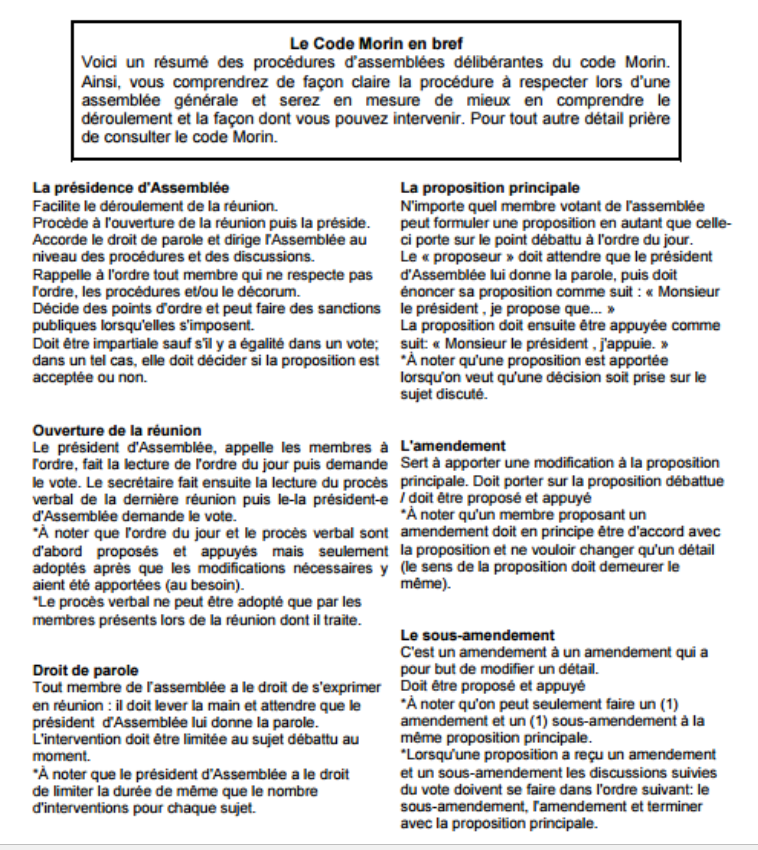
\includegraphics[width = 16cm]{Code1.PNG}
%\newpage
%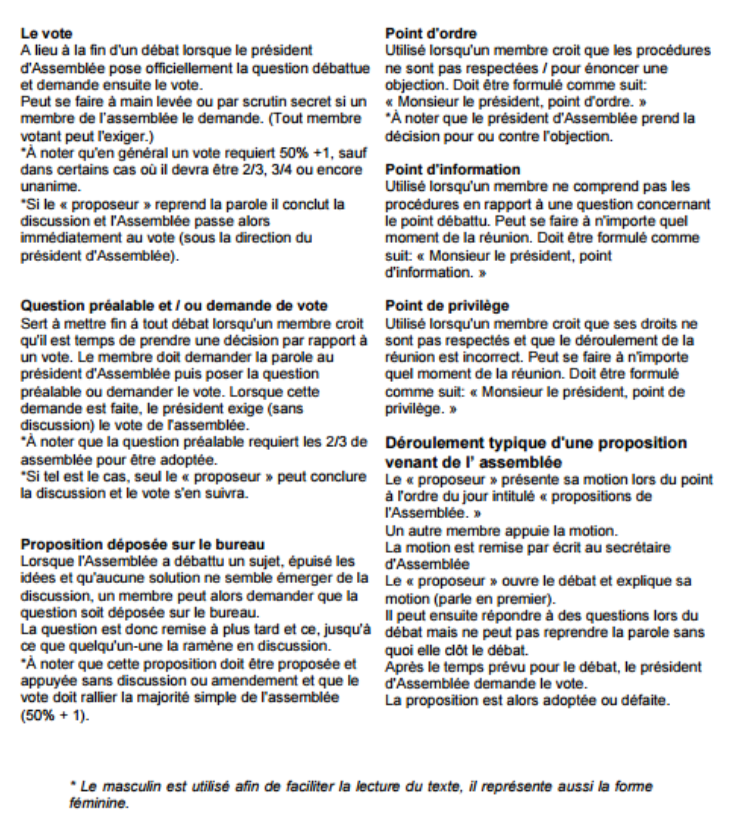
\includegraphics[width = 16cm]{Code2.PNG}
%\newpage